\documentclass{report}

%%%%%%%%%%%%%%%%%%%%%%%%%%%%%%%%%
% PACKAGE IMPORTS
%%%%%%%%%%%%%%%%%%%%%%%%%%%%%%%%%


\usepackage{graphicx, float}
\graphicspath{{res/}}
\usepackage{tikz}     % tableofcontents
\usepackage{titletoc} % tableofcontents
\usepackage{mathptmx}
\usepackage[skip=0.8em, indent=0pt]{parskip}

\usepackage[hidelinks]{hyperref}


%%%%%%%%%%%%%%%%%%%%%%%%%%%%%%
% MODIFIED COMMANDS
%%%%%%%%%%%%%%%%%%%%%%%%%%%%%%


\newcommand{\bcite}[1]{\textbf{\cite{#1}}}
\renewcommand{\footnoterule}{\vfill\kern -3pt \hrule width 0.4\columnwidth \kern 2.6pt}

\renewcommand{\abstractname}{Zusammenfassung}
\renewcommand{\contentsname}{Inhalt}
\newcommand{\replacechaptername}{Kapitel}
\renewcommand{\chaptername}{\replacechaptername}
\renewcommand{\bibname}{Quellenverzeichnis}
\newcommand{\replacepagename}{Seite}


%%%%%%%%%%%%%%%%%%%%%%%%%%%%%%
% SELF MADE COLORS
%%%%%%%%%%%%%%%%%%%%%%%%%%%%%%


\definecolor{doc}{RGB}{0,60,110}


%%%%%%%%%%%%%%%%%%%%%%%%%%%%%%%%%%%%%%%%%%%
% TABLE OF CONTENTS
%%%%%%%%%%%%%%%%%%%%%%%%%%%%%%%%%%%%%%%%%%%


\contentsmargin{0cm}
\titlecontents{chapter}[3.7pc]
{\addvspace{30pt}
	\begin{tikzpicture}[remember picture, overlay]
		\draw[fill=doc!60,draw=doc!60] (-7,-.1) rectangle (-0.9,.5);
		\pgftext[left,x=-3.5cm,y=0.2cm]{\color{white}\Large\sc\bfseries \replacechaptername\ \thecontentslabel};
	\end{tikzpicture}\color{doc!60}\large\sc\bfseries}
{}
{}
{\;\titlerule\;\large\sc\bfseries \replacepagename\space\thecontentspage
	\begin{tikzpicture}[remember picture, overlay]
		\draw[fill=doc!60,draw=doc!60] (2pt,0) rectangle (4,0.1pt);
	\end{tikzpicture}}
\titlecontents{section}[3.7pc]
{\addvspace{2pt}}
{\contentslabel[\thecontentslabel]{2pc}}
{}
{\hfill\small \thecontentspage}
[]
\titlecontents{subsection}[4.7pc]
{\addvspace{-1pt}\small}
{}
{}
{\hfill\small \thecontentspage}
[]
\titlecontents{bibliography}[3.7pc]
{\addvspace{30pt}
	\color{doc!60}\large\sc\bfseries}
{}
{}
{\;\titlerule\;\large\sc\bfseries \replacepagename\space\thecontentspage
	\begin{tikzpicture}[remember picture, overlay]
		\draw[fill=doc!60,draw=doc!60] (2pt,0) rectangle (4,0.1pt);
	\end{tikzpicture}}

\makeatletter
\renewcommand{\tableofcontents}{
	\chapter*{
	  \vspace*{-20\p@}
	  \begin{tikzpicture}[remember picture, overlay]
		  \pgftext[right,x=15cm,y=0.2cm]{\color{doc!60}\Huge\sc\bfseries \contentsname};
		  \draw[fill=doc!60,draw=doc!60] (13.5,-.75) rectangle (20,1);
		  \clip (13.5,-.75) rectangle (20,1);
		  \pgftext[right,x=15cm,y=0.2cm]{\color{white}\Huge\sc\bfseries \contentsname};
	  \end{tikzpicture}}
	\@starttoc{toc}}
\makeatother


\input{macros}
\input{letterfonts}

\title{\Huge{Theoretische Informatik}\\Testate}
\author{\huge{Silas Alexander Kraume}\\sikra111}
\date{}


\begin{document}

\maketitle
\newpage% or \cleardoublepage
% \pdfbookmark[<level>]{<title>}{<dest>}
\pdfbookmark[section]{\contentsname}{toc}
\tableofcontents
\pagebreak

\chapter{}
\section{Aufgabe 1}


\begin{algorithm}[H]
% \KwIn{This is some input}
% \KwOut{This is some output}
\SetAlgoLined
\SetNoFillComment
% \tcc{This is a comment}
\vspace{3mm}
\uIf{C} {
  \uIf{C} {
    S
  }
}
\Else {
    S
}
\caption{}
\end{algorithm}

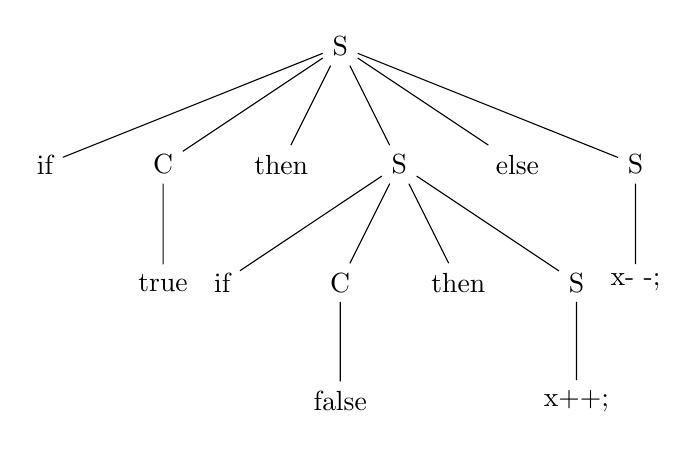
\begin{tikzpicture}
\node {S}
  child { node{if} }
  child { node{C} 
    child { node{true} } }
  child { node{then} }
  child { node{S} 
    child { node{if} }
    child { node{C} 
      child { node{false} } }
    child { node{then} }
    child { node{S} 
      child { node{x++;} } } }
  child { node{else} }
  child { node{S}
    child{ node{x- -;} } }
  ;
\end{tikzpicture}

\begin{algorithm}[H]
% \KwIn{This is some input}
% \KwOut{This is some output}
\SetAlgoLined
\SetNoFillComment
% \tcc{This is a comment}
\vspace{3mm}
\uIf{C} {
  \uIf{C} {
    S
  }
  \Else {
    S
  }
}
\caption{}
\end{algorithm}

\begin{tikzpicture}
\node {S}  [sibling distance=3cm]
  child { node{if} }
  child { node{C} 
    child{ node{true} } }
  child { node{then} }
  child { node{S}   [sibling distance=1cm]
    child{ node{if} } 
    child{ node{C} 
      child{ node{false} } } 
    child{ node{then} } 
    child{ node{S} 
      child{ node{x++;} } } 
    child{ node{else} } 
    child{ node{S} 
    child{ node{x- -;} } } }
  ;
\end{tikzpicture}

Wort:%
\framebox[1.1\width]{if true then if false then x++; else x- -;} \par

\section{Aufgabe 2}

\leftline{a)}

% \vspace{0.5cm}
$\newline$
\leftline{R$\textsubscript{1}$: [0-9]}

\begin{tikzpicture}[>=stealth, auto, node distance=2.8cm,
  thick, accepting/.style={double distance=1.5pt, outer sep=0.75pt+\pgflinewidth}]
  \node[state, initial] (z0) {};
  \node[state, accepting] (z1) [right of=z0] {};
  \path[->] (z0) edge node {[0-9]} (z1);
\end{tikzpicture}

\vspace{0.5cm}
\leftline{R$\textsubscript{2}$: [0-9]$\textsuperscript{*}$}

\begin{tikzpicture}[>=stealth, auto, node distance=2.8cm,
  thick, accepting/.style={double distance=1.5pt, outer sep=0.75pt+\pgflinewidth}]
  \node[state, initial, accepting] (z0) {};
  \node[state, initial] (z1) [below of=z0] {};
  \node[state, accepting] (z2) [right of=z1] {};
  \path[->] (z1) edge node {[0-9]} (z2);
  \path[->] (z1) edge node {[0-9]} (z0);
  \path[-stealth] (z1) edge[loop below] node[below] {[0-9]} ();
\end{tikzpicture}

\vspace{0.5cm}
\leftline{R$\textsubscript{3}$: R$\textsubscript{1}$R$\textsubscript{2}$}

\begin{tikzpicture}[>=stealth, auto, node distance=2.8cm,
  thick, accepting/.style={double distance=1.5pt, outer sep=0.75pt+\pgflinewidth}]
  \node[state, initial] (z0) {$z_0$};
  \node[state, accepting] (z1) [right of=z0] {$z_1$};
  \node[state, accepting] (z2) [below of=z1] {$z_2$};
  \node[state] (z3) [below of=z2] {$z_3$};
  \node[state, accepting] (z4) [right of=z3] {$z_4$};
  \path[->] (z0) edge node {[0-9]} (z1);
  \path[->] (z0) edge node {[0-9]} (z2);
  \path[->] (z0) edge node[left] {[0-9]} (z3);
  \path[-stealth] (z3) edge[loop below] node[below] {[0-9]} ();
  \path[->] (z3) edge node {[0-9]} (z4);
  \path[->] (z3) edge node[right] {[0-9]} (z2);
  % \path[-stealth] (z0) edge[loop below] node[below] {[0-9]} ();
\end{tikzpicture}

\leftline{M = ($\Sigma, Z, \delta, S, E$)}
\leftline{$Z = \{ z_0, z_1, z_2, z_3, z_4 \}$, $S = \{ z_0 \}$, $E = \{ z_1, z_2, z_4 \}$}

\newpage

\leftline{b)}

\begin{tikzpicture}[>=stealth, auto, node distance=2.8cm,
  thick, accepting/.style={double distance=1.5pt, outer sep=0.75pt+\pgflinewidth}]
  \node[state, initial] (z0) {\{$z_0$\}};
  \node[state, accepting] (z1) [right of=z0] {$\{z_1, z_2, z_3\}$};
  \node[state, accepting] (z2) [right of=z1] {$\{z_2, z_3, z_4\}$};
  \path[->] (z0) edge node {[0-9]} (z1);
  \path[->] (z1) edge node {[0-9]} (z2);
  \path[-stealth] (z2) edge[loop below] node[below] {[0-9]} ();
\end{tikzpicture}

\leftline{N = ($\Sigma, Z, \delta, S, F$)}
\leftline{$Z = \{ z_0, \{z_1, z_2, z_3\}, \{z_2, z_3, z_4\}, z_3\}$, $S = z_0$, $E = \{ \{z_1, z_2, z_3\}, \{z_2, z_3, z_4\}, z_3 \}$}

\leftline{c)}

\begin{tikzpicture}[>=stealth, auto, node distance=2.8cm,
  thick, accepting/.style={double distance=1.5pt, outer sep=0.75pt+\pgflinewidth}]
  \node[state, initial] (z0) {$z_0$};
  \node[state, accepting] (z1) [right of=z0] {$z_1$};
  \path[->] (z0) edge node {[0-9]} (z1);
  \path[-stealth] (z1) edge[loop below] node[below] {[0-9]} ();
\end{tikzpicture}

\leftline{d)}

\leftline{$\alpha$ = [0-9][0-9]$\textsuperscript{*}$}
\leftline{$\beta$ = ws ws$\textsuperscript{*}$}
\leftline{$\gamma$ = [a-zA-Z][a-zA-Z0-9]$\textsuperscript{*}$}

\begin{tikzpicture}[>=stealth, auto, node distance=2.8cm,
  thick, accepting/.style={double distance=1.5pt, outer sep=0.75pt+\pgflinewidth}]
  \node[state, initial] (z0) {$z_0$};
  \node[state, accepting] (z1) [right of=z0] {$z_1$};
  \node[state, accepting] (z2) [above of=z1] {$z_2$};
  \node[state, accepting] (z3) [below of=z1] {$z_3$};
  \path[->] (z0) edge node {$\alpha$} (z1);
  \path[-stealth] (z1) edge[loop below] node[below] {$\alpha$} ();
  \path[->] (z0) edge node {$\beta$} (z2);
  \path[-stealth] (z2) edge[loop below] node[below] {$\beta$} ();
  \path[->] (z0) edge node {$\gamma$} (z3);
  \path[-stealth] (z3) edge[loop below] node[below] {$\gamma$} ();
\end{tikzpicture}

\newpage
\section{Aufgabe 3}

\leftline{a) $\alpha$ steht beliebig oft, aber mindestens einmal, hintereinander:}
\centerline{$\alpha$\textsuperscript{+} $\equiv$ $\alpha$($\alpha$)\textsuperscript{*}}
\centerline{$\textit{L}$($\alpha$($\alpha$)\textsuperscript{*}) = $\textit{L}$($\alpha$)$\textit{L}$($\alpha$\textsuperscript{*}) = $\textit{L}$($\alpha$)$\textit{L}$($\alpha$)\textsuperscript{*} = \{$\alpha$x $\vert$ x $\in$ $\alpha$\textsuperscript{*} \}}
\vspace{0.5cm}

\leftline{b) $\alpha$ tritt einmal oder gar nicht auf:}
\centerline{$\alpha$? $\equiv$ ($\lambda$ + $\alpha$)}
\centerline{$\textit{L}$($\lambda$ + $\alpha$) = $\textit{L}$($\lambda$) $\cup$ $\textit{L}$($\alpha$) = \{$\lambda$\} $\cup$ $\textit{L}$($\alpha$)}
\vspace{0.5cm}

\leftline{c) für eine natürliche Zahl \textit{n} wird $\alpha$ genau \textit{n}-mal wiederholt:}
\centerline{$\alpha$\textsuperscript{\textit{n}} $\equiv$ $\underbrace{\alpha \alpha \cdot \cdot \cdot \alpha}_{\text{\textit{n} mal} }$}
\centerline{$\textit{L}$$\left(\underbrace{\alpha \alpha \cdot \cdot \cdot \alpha}_{\text{\textit{n} mal} }\right)$ = $\underbrace{\textit{L}\left(\alpha\right) \textit{L}\left(\alpha\right) \cdot \cdot \cdot \textit{L}\left(\alpha\right)}_{\text{\textit{n} mal} }$}

\chapter{}
\section{Aufgabe 1}
Angenommen G sei regulär. Dann existiert nach dem Pumping-Lemma eine Zahl n $\geq$ 1, so dass für alle Wörter x $\in$ L(G) mit
$\left\lvert x\right\rvert$ $\geq$ n eine Zerlegung x = uvw mit

1. $\left\lvert uv\right\rvert$ $\leq$ n

2. $\left\lvert v\right\rvert$ $\geq$ 1

3. $\forall\textit{i}$ $\geq$ 0. uv$\textsuperscript{\textit{i}}$w $\in$ L(G)

$\newline$
Wähle x = $\underbrace{\text{\lparen\lparen}\cdot\cdot\cdot\text{\lparen\lparen}}_{\text{\textit{n} mal}}$ a $\underbrace{\text{ + a\rparen}\text{ + a\rparen}\cdot\cdot\cdot\text{ + a\rparen}}_{\text{\textit{n} mal}}$
$\in$ L(G) mit $\left\lvert x\right\rvert$ = 2n + 1 $\geq$ n.
$\newline$
Sei x = uvw = $\text{\lparen\textsuperscript{n}}$a$\left(\text{+a\rparen}\right)\textsuperscript{n}$, also uv = $\text{\lparen\textsuperscript{n}}$.
$\newline$
Aus uv = $\text{\lparen\textsuperscript{n}}$ folgt ebenfalls v = $\text{\lparen\textsuperscript{i}}$ für ein i $\leq$ n
und entsprechend u = $\text{\lparen\textsuperscript{j}}$ für ein j = n-i.
$\newline$
Für jedes k$\in\mathbb{N}$ ${\displaystyle >\,}$ n gilt: uv$\textsuperscript{k}$w $\notin$ L(G).
$\newline$
Insbesondere gilt für k = 0:  uv$\textsuperscript{k}$w = uv$\textsuperscript{0}$w = uw $\notin$ L(G).
$\newline$
Es folgt: G ist nicht regulär!

$\rightline{\qed}$

\section{Aufgabe 2}

\leftline{x = uv$\textsuperscript{3}$w = abcdbcdbcdbe $\in$ $\textit{L(M)}$, $\left\lvert x\right\rvert$ $\geq$ $\textit{p}$}
\leftline{1. $\left\lvert uv\right\rvert$ $\leq$ $\textit{p}$}
\leftline{2. $\left\lvert v\right\rvert$ $\geq$ 1}
\leftline{3. $\forall\textit{i}$ $\geq$ 0. uv$\textsuperscript{\textit{i}}$w $\in$ $\textit{L(M)}$}

\leftline{$\Rightarrow $ u = ab, v = cdb, w = e}

\leftline{$\Rightarrow $ uv$\textsuperscript{\textit{i}}$w = ab(cdb)$\textsuperscript{\textit{i}}$e $\in$ $\textit{L(M)}$ }

\vspace{0.5cm}
\section{Aufgabe 3}

\leftline{a) ist regulär, ein einfacher DFA für den entsprechenden Ausdruck ist trivial.}
\leftline{b) + c) nicht regulär, denn HTML und Java sind endlos erweiterbar, erlauben willkürlich verschachtelte/rekursive Strukturen.}

\newpage
\section{Aufgabe 4}

\leftline{a)}

1. Entferne alle von $z_0$ aus nicht erreichbaren Zustände aus $\textit{Z}$.
$\newline$
Alle Zustände sind von $z_0$ aus erreichbar.
$\newline\newline$
2. Erstelle eine Tabelle aller (ungeordneten) Zustandspaare $\{z, z'\}$ von $\textit{M}$ mit $z \neq z'$. $\newline$
3. Markiere alle Paare $\{z, z'\}$ mit $z \in \textit{F} \Leftrightarrow z' \notin \textit{F}$. $\newline$
$\newline$

\begin{center}
  \begin{tabular}{|c||c|c|c|c|} %Für weitere Spalten hier mit c ergänzen, | sorgt für die Trennlinien
    \hline
    & $z_0$ & $z_1$ & $z_2$ & $z_3$ \\
    \hline
    \hline
    $z_4$ & & $X$ & $X$ & $X$ \\
    \hline
    $z_3$ & $X$ & & & $-$ \\
    \hline
    $z_2$ & $X$ & & $-$ & $-$ \\
    \hline
    $z_1$ & $X$ & $-$ & $-$ & $-$ \\
    \hline
  \end{tabular}
\end{center}

$\newline$
4. Sei $\{z, z'\}$ ein unmarkiertes Paar. Prüfe für jedes a $\in \Sigma$, ob $\{\sigma$($z, a$)$, \sigma$($z', a$)$\}$ bereits markiert ist.
Ist mindestens ein Test erfolgreich, so markiere auch $\{z, z'\}$.
$\newline$
5. Wiederhole Schritt 4, bis keine Änderung mehr eintritt.
$\newline$

\centerline{$\{\sigma$($z_1, 0$)$, \sigma$($z_3, 0$)$\}$ = $\{z_2, z_4\}$}
\centerline{$\{\sigma$($z_2, 0$)$, \sigma$($z_3, 0$)$\}$ = $\{z_2, z_4\}$}
\centerline{$\{\sigma$($z_1, 1$)$, \sigma$($z_2, 1$)$\}$ = $\{z_0, z_2\}$}

\begin{center}
  \begin{tabular}{|c||c|c|c|c|} %Für weitere Spalten hier mit c ergänzen, | sorgt für die Trennlinien
    \hline
    & $z_0$ & $z_1$ & $z_2$ & $z_3$ \\
    \hline
    \hline
    $z_4$ & & $X$ & $X$ & $X$ \\
    \hline
    $z_3$ & $X$ & $X$ & $X$ & $-$ \\
    \hline
    $z_2$ & $X$ & $X$ & $-$ & $-$ \\
    \hline
    $z_1$ & $X$ & $-$ & $-$ & $-$ \\
    \hline
  \end{tabular}
\end{center}

$\newline$
6. Bilde maximale Mengen paarweise nicht disjunkter unmarkierter Zustandspaare und verschmelze jeweils alle Zustände einer Menge zu einem neuen Zustand.
$\newline$
Verschmelze $z_0$ und $z_4$ zu $z\textsubscript{04}$.

M' = ($\Sigma$, Z', $\sigma$', $z\textsubscript{04}$, F')

$\Sigma$ = $\{0, 1\}$

Z' = $\{z\textsubscript{04}, z_1, z_2, z_3\}$

F' = $\{z\textsubscript{04}\}$

\begin{center}
  \begin{tabular}{|c||c|c|c|c|} %Für weitere Spalten hier mit c ergänzen, | sorgt für die Trennlinien
    \hline
    $\sigma$' & $z\textsubscript{04}$ & $z_1$ & $z_2$ & $z_3$ \\
    \hline
    \hline
    $0$ & $z_3$ & $z_2$ & $z_2$ & $z\textsubscript{04}$ \\
    \hline
    $1$ & $z_1$ & $z\textsubscript{04}$ & $z_2$ & $z_2$ \\
    \hline
  \end{tabular}
\end{center}

\newpage

M:
$\newline$

\begin{tikzpicture}[>=stealth, auto, node distance=2.8cm,
  thick, accepting/.style={double distance=1.5pt, outer sep=0.75pt+\pgflinewidth}]
  \node[state, initial, accepting] (z0) {$z_0$};
  \node[state, accepting] (z4) [right of=z0] {$z_4$};
  \node[state] (z3) [above of=z4] {$z_3$};
  \node[state] (z1) [below of=z4] {$z_1$};
  \node[state] (z2) [right of=z4] {$z_2$};
  \path[->] (z0) edge node {$0$} (z3);
  \path[->] (z0) edge node {$1$} (z1);
  \path[->] (z1) edge node {$0$} (z2);
  \path[->] (z1) edge node {$1$} (z0);
  \path[-stealth] (z2) edge[loop below] node[below] {$0, 1$} ();
  \path[->] (z3) edge node {$0$} (z4);
  \path[->] (z3) edge node {$1$} (z2);
  \path[->] (z4) edge node {$0$} (z3);
  \path[->] (z4) edge node {$1$} (z1);
\end{tikzpicture}



M':
$\newline$

\begin{tikzpicture}[>=stealth, auto, node distance=2.8cm,
  thick, accepting/.style={double distance=1.5pt, outer sep=0.75pt+\pgflinewidth}]
  \node[state, initial, accepting] (z0) {$z\textsubscript{04}$};
  \node[state] (z3) [above of=z4] {$z_3$};
  \node[state] (z1) [below of=z4] {$z_1$};
  \node[state] (z2) [right of=z4] {$z_2$};
  \path[->] (z0) edge node {$0$} (z3);
  \path[->] (z0) edge node {$1$} (z1);
  \path[->] (z1) edge node {$0$} (z2);
  \path[->] (z1) edge node {$1$} (z0);
  \path[-stealth] (z2) edge[loop below] node[below] {$0, 1$} ();
  \path[->] (z3) edge node {$0$} (z0);
  \path[->] (z3) edge node {$1$} (z2);
\end{tikzpicture}

$\newline$
\leftline{b)}
Äquivalenzklassen:

[$\lambda$] = \{$\lambda$, 00, 11, \dots\}

[0]

[1]

[01] = [10]

$\newline$
\leftline{c)}
Man kann folgende Zustände zusammen legen:

$z_1$ und $z_6$

$z_2$ und $z_4$ und $z_7$

\chapter{}

\section{Aufgabe 1}

\leftline{a)}

N\textsubscript{$\lambda$} = \{C\}, da C $\rightarrow \lambda \in$ P\textsubscript{1}
$\newline$
N\textsubscript{$\lambda$} = \{C, D\}, da D $\rightarrow$ CCC $\rightarrow \lambda \in$ P\textsubscript{1}
$\newline$
\begin{align*}
  P'\textsubscript{1}= \{ S &\to AD\ |\ DA\ |\ A,\\
  A &\to BC\ |\ B,\\
  B &\to S1\ |\ 0,\\
  C &\to 1,\\
  D &\to AB\ |\ CCC\ |\ 0C\ |\ CC\ |\ C\ |\ 0\}
\end{align*}

\leftline{b)}
$\newline$
Zyklus: B $\to$ C $\to$ D $\to$ B $\dots$
$\newline$
N'\textsubscript{2} = \{S, A, X\}
\begin{align*}
  P'\textsubscript{2}= \{ S &\to AXXS\ |\ a,\\
  A &\to a\ |\ aX,\\
  X &\to bA,\\
  X &\to AX\ |\ c,\\
  X &\to d\} \\
  = \{ S &\to AXXS\ |\ a,\\
  A &\to a\ |\ aX,\\
  X &\to bA\ |\ AX\ |\ c\ |\ d\}
\end{align*}

\leftline{c)}
$\newline$
Zyklus: /
$\newline$
S(1), A(2), B(3), C(4), D(5)
\begin{align*}
  P'\textsubscript{3}= \{ S &\to ABCS\ |\ a,\\
  A &\to a\ |\ aB,\\
  B &\to Ad\ |\ d\ |\ c\ |\ bA,\\
  C &\to Ad\ |\ d\ |\ c,\\
  D &\to d\}.
\end{align*}

\newpage

\leftline{d)}
$\newline$
$\lambda$-frei \checkmark
$\newline$
keine einfachen Regel \checkmark
$\newline$
A $\to$ a und B $\to$ b werden übernommen.
$\newline$
X\textsubscript{a}, X\textsubscript{b} einführen:
\begin{align*}
  P'\textsubscript{4}= \{ S &\to ABAS\ |\ X_aX_b,\\
  A &\to X_aA\ |\ a,\\
  B &\to b\ |\ X_aX_bX_b,\\
  X_a &\to a,\\
  X_b &\to b\}.
\end{align*}
$\newline$
Nichtterminalketten ersetzen:
\begin{align*}
  P''\textsubscript{4}= \{ S &\to AC_0\ |\ X_aX_b,\\
  A &\to X_aA\ |\ a,\\
  B &\to b\ |\ X_aC_2,\\
  X_a &\to a,\\
  X_b &\to b, \\
  C_0 &\to BC_1, \\
  C_1 &\to AS, \\
  C_2 &\to X_bX_b\}.
\end{align*}
$\newline$
N'\textsubscript{4} = \{S, A, B, X\textsubscript{a}, X\textsubscript{b}, C\textsubscript{0}, C\textsubscript{1}, C\textsubscript{2} \}


\section{Aufgabe 2}

\leftline{a)}
\begin{center}
  $\begin{array}{c|c|c|c|c|c|c|}
  i & 1      & 2    & 3    & 4      & 5    & 6        \\ \hline
  5 & S, S_2                                          \\ \cline{1-3}
  4 &        & C_2                                    \\ \cline{1-4}
  3 & S      &      & T_2                             \\ \cline{1-5}
  2 &        & C_2  &      & S_2                      \\ \cline{1-6}
  1 &        &      & T_2  &        & E_2             \\ \hline
  0 & I      & C    & T    & S      & E    & S        \\ \hline
  j & if     & true & then & $x++;$ & else & x$-$$-$; 
  \end{array}$
\end{center}

\leftline{b)}
\begin{center}
  $\begin{array}{c|c|c|c|c|c|}
  i & 1      & 2    & 3    & 4      & 5          \\ \hline
  4 &                                            \\ \cline{1-3}
  3 & S  &                                       \\ \cline{1-4}
  2 &    & C_2  &                                \\ \cline{1-5}
  1 &    &      & T_2  &                         \\ \hline
  0 & I  & C    & T    & S      & E              \\ \hline
  j & if & true & then & $x++;$ & else
  \end{array}$
\end{center}

\newpage

\section{Aufgabe 3}

\leftline{a)}
$\newline$

L = \{$\left(ab\right)$\textsuperscript{m}c\textsuperscript{2m} $|$ 1 $\le$ m $\in \mathbb{N} $\}

$\newline$
\leftline{b)}
$\newline$

$\bullet$ DPDAs sind in (N)PDAs überführbar.

$\bullet$ Die Sprache, die ein DPDA akzeptiert ist eine Teilmenge der Sprache, die ein PDA akzeptiert.

$\bullet$ DPDA hat zusätzlich Endzustände definiert.

$\bullet$ DPDA akzeptiert eine Eingabe per Endzustand, nicht leerem Stack.

$\bullet$ DPDAs sind deterministisch, haben also eindeutig bestimmte Übergänge.

\section{Aufgabe 4}

M = (\{a, b\}, \{a, b, S, A, B\}, \{z\}, $\delta$, z, S)
$\newline$
$\delta$:

z$\lambda$S $\to$ zABAS

z$\lambda$S $\to$ zab

z$\lambda$A $\to$ zaA

z$\lambda$A $\to$ za

z$\lambda$B $\to$ zb

z$\lambda$B $\to$ zabb
$\newline$

zaa $\to$ z $\lambda$

zbb $\to$ z $\lambda$

\chapter{}

\section{Aufgabe 1}

\leftline{a)}
\begin{eqnarray}
  z_0<div><div><\textit{/}div><div><\textit{/}div><\textit{/}div><div>\widehat{<\textit{/}div>} & \vdash_{M} \nonumber \\
  \widehat{<div>}z_1<div><\textit{/}div><div><\textit{/}div><\textit{/}div><div>\widehat{<\textit{/}div>} & \vdash_{M} \nonumber \\
  \widehat{<div>}<div>z_1<\textit{/}div><div><\textit{/}div><\textit{/}div><div>\widehat{<\textit{/}div>} & \vdash_{M} \nonumber \\
  \widehat{<div>}z_2<div>\square<div><\textit{/}div><\textit{/}div><div>\widehat{<\textit{/}div>} & \vdash_{M} \nonumber \\
  \widehat{<div>}\square z_1\square<div><\textit{/}div><\textit{/}div><div>\widehat{<\textit{/}div>} & \vdash_{M} \nonumber \\
  \widehat{<div>}\square\square z_1<div><\textit{/}div><\textit{/}div><div>\widehat{<\textit{/}div>} & \vdash_{M} \nonumber \\
  \widehat{<div>}\square\square<div>z_1<\textit{/}div><\textit{/}div><div>\widehat{<\textit{/}div>} & \vdash_{M} \nonumber \\
  \widehat{<div>}\square\square z_2<div>\square<\textit{/}div><div>\widehat{<\textit{/}div>} & \vdash_{M} \nonumber \\
  \widehat{<div>}\square\square\square z_1\square<\textit{/}div><div>\widehat{<\textit{/}div>} & \vdash_{M} \nonumber \\
  \widehat{<div>}\square\square\square\square z_1<\textit{/}div><div>\widehat{<\textit{/}div>} & \vdash_{M} \nonumber \\
  \widehat{<div>}\square\square\square z_2\square\square<div>\widehat{<\textit{/}div>} & \vdash_{M} \nonumber \\
  \widehat{<div>}\square\square z_2\square\square\square<div>\widehat{<\textit{/}div>} & \vdash_{M} \nonumber \\
  \widehat{<div>}\square z_2\square\square\square\square<div>\widehat{<\textit{/}div>} & \vdash_{M} \nonumber \\
  \widehat{<div>}z_2\square\square\square\square\square<div>\widehat{<\textit{/}div>} & \vdash_{M} \nonumber \\
  z_2\widehat{<div>}\square\square\square\square\square<div>\widehat{<\textit{/}div>} & \vdash_{M} \nonumber \\
  \widehat{<div>}z_4\square\square\square\square\square<div>\widehat{<\textit{/}div>} & \vdash_{M} \nonumber \\
  \widehat{<div>}\square z_4\square\square\square\square<div>\widehat{<\textit{/}div>} & \vdash_{M} \nonumber \\
  \widehat{<div>}\square\square z_4\square\square\square<div>\widehat{<\textit{/}div>} & \vdash_{M} \nonumber \\
  \widehat{<div>}\square\square\square z_4\square\square<div>\widehat{<\textit{/}div>} & \vdash_{M} \nonumber \\
  \widehat{<div>}\square\square\square\square z_4\square<div>\widehat{<\textit{/}div>} & \vdash_{M} \nonumber \\
  \widehat{<div>}\square\square\square\square\square z_4<div>\widehat{<\textit{/}div>} & \vdash_{M} \nonumber \\
  \widehat{<div>}\square\square\square\square\square\widehat{<div>}z_1\widehat{<\textit{/}div>} & \vdash_{M} \nonumber \\
  \widehat{<div>}\square\square\square\square\square z_3\widehat{<div>}\widehat{<\textit{/}div>} & \vdash_{M} \nonumber \\
  \widehat{<div>}\square\square\square\square\square z_e\widehat{<div>}\widehat{<\textit{/}div>} \nonumber
\end{eqnarray}

\newpage
\leftline{b)}

$a \widehat{=} <div>$

$b \widehat{=} \widehat{<div>}$

$c \widehat{=} <\textit{/}div>$

$d \widehat{=} \widehat{<\textit{/}div>}$


\begin{tikzpicture}[>=stealth, auto, node distance=2.8cm,
  thick, accepting/.style={double distance=1.5pt, outer sep=0.75pt+\pgflinewidth}]
  \node[state, initial] (z0) {$z\textsubscript{0}$};
  \node[state] (z1) [right of=z0] {$z_1$};
  \node[state] (z3) [above of=z1] {$z_3$};
  \node[state, accepting] (ze) [right of=z3] {$z_e$};
  \node[state] (z4) [right of=z1] {$z_4$};
  \node[state] (z2) [below of=z4] {$z_2$};
  \path[->] (z0) edge node {$a,b,R$} (z1);
  \path[-stealth] (z0) edge[loop below] node[below] {$\square,\square,N$} ();
  \path[-stealth] (z1) edge[loop below] node[below] {$a\textit{/}\square,a\textit{/}\square,R$} ();
  \path[->] (z1) edge node {$d,d,L$} (z3);
  \path[->] (z1) edge node {$c,\square,L$} (z2);
  \path[->] (z2) edge node {$a,\square,R$} (z1);
  \path[-stealth] (z2) edge[loop below] node[below] {$\square,\square,L$} ();
  \path[->] (z2) edge node[right] {$b,b,R$} (z4);
  \path[->] (z3) edge node {$b,b,N$} (ze);
  \path[-stealth] (z3) edge[loop left] node[left] {$\square,\square,L$} ();
  \path[->] (z4) edge node {$a,b,R$} (z1);
  \path[-stealth] (z4) edge[loop right] node[right] {$\square,\square,R$} ();
\end{tikzpicture}

$\newline$
L(M) akzeptiert Eingaben, bei denen jedes öffnende div ein matchendes schließendes div besitzt.
Hierbei hat das letzte (schließende) div bereits einen Hut, als Vorraussetung für einen LBA, aus diesem
Grund wird auch das erste (öffnende) div mit einem Hut markiert. Die TM akzeptiert zudem die leere Eingabe.

$\newline$
\leftline{c)}

LBA:

hat spezifisches Start- und Endsymbol (bzw. verdoppeltes Eingabealphabet).

verlässt den Bereich des Eingabewortes nicht.

verändert die Länge der auf dem Band stehenden Eingabe nicht.

\leftline{d)}

Ja, M ist ein LBA.

\newpage

\section{Aufgabe 2}

f(x) = x mod 3

M = $\left(\Sigma,\Gamma,Z,\delta,z_0,\square,F\right)$

$\Sigma = \lbrace 0,1,2,3,4,5,6,7,8,9\rbrace$

$\Gamma = \lbrace 0,1,2,3,4,5,6,7,8,9,\square\rbrace$

Z = $\lbrace z_0,z_1,z_2,z_e\rbrace$

F = $\lbrace z_e\rbrace$

\begin{center}
  $\begin{array}{c|c|c|c|}
  \delta  & z_0                        & z_1                        & z_2                        \\ \hline
  0       & \left(z_0,\square,R\right) & \left(z_1,\square,R\right) & \left(z_2,\square,R\right) \\ \hline
  1       & \left(z_1,\square,R\right) & \left(z_2,\square,R\right) & \left(z_0,\square,R\right) \\ \hline
  2       & \left(z_2,\square,R\right) & \left(z_0,\square,R\right) & \left(z_1,\square,R\right) \\ \hline
  3       & \left(z_0,\square,R\right) & \left(z_1,\square,R\right) & \left(z_2,\square,R\right) \\ \hline
  4       & \left(z_1,\square,R\right) & \left(z_2,\square,R\right) & \left(z_0,\square,R\right) \\ \hline
  5       & \left(z_2,\square,R\right) & \left(z_0,\square,R\right) & \left(z_1,\square,R\right) \\ \hline
  6       & \left(z_0,\square,R\right) & \left(z_1,\square,R\right) & \left(z_2,\square,R\right) \\ \hline
  7       & \left(z_1,\square,R\right) & \left(z_2,\square,R\right) & \left(z_0,\square,R\right) \\ \hline
  8       & \left(z_2,\square,R\right) & \left(z_0,\square,R\right) & \left(z_1,\square,R\right) \\ \hline
  9       & \left(z_0,\square,R\right) & \left(z_1,\square,R\right) & \left(z_2,\square,R\right) \\ \hline
  \square & \left(z_e,0,N\right)       & \left(z_e,1,N\right)       & \left(z_e,2,N\right)       \\ \hline
  \end{array}$
\end{center}

\section{Aufgabe 3}
$\newline$

P1: $\newline$
Kein LOOP, wegen Keyword WHILE. $\newline$
Ist WHILE. $\newline$
Kein GOTO, wegen Keyword DO. $\newline$

P2: $\newline$
Kein LOOP, weil $x_2$ in Loop + ";" vor END. $\newline$
Kein WHILE, weil $x_2$ in Loop + ";" vor END. $\newline$
Kein GOTO, wegen Keyword DO. $\newline$

P3: $\newline$
Kein LOOP, weil $x_0 := x_1;$ (anstatt $x_0 := x_1 $+$ 0;$). $\newline$
Kein WHILE, weil $x_0 := x_1;$ (anstatt $x_0 := x_1 $+$ 0;$). $\newline$
Kein GOTO, wegen Keyword DO. $\newline$

P4: $\newline$
Kein LOOP, weil $x_2$ in Loop. $\newline$
Kein WHILE, weil $x_2$ in Loop. $\newline$
Kein GOTO, wegen Keyword DO. $\newline$

P5: $\newline$
Kein LOOP, weil $x_1$ in Loop. $\newline$
Kein WHILE, weil $x_1$ in Loop. $\newline$
Kein GOTO, wegen Keyword DO. $\newline$

P6: $\newline$
Kein LOOP, wegen Keyword WHILE. $\newline$
Kein WHILE, weil ";" vor END. $\newline$
Kein GOTO, wegen Keyword DO. $\newline$

P7: $\newline$
Ist LOOP. $\newline$
Ist WHILE, weil es LOOP ist.$\newline$
Kein GOTO, wegen Keyword DO. $\newline$

P8: $\newline$
Kein LOOP, wegen Keyword WHILE. $\newline$
Kein WHILE, wegen Keyword GOTO. $\newline$
Kein GOTO, wegen Keyword DO. $\newline$

P9: $\newline$
Kein LOOP, wegen Keyword GOTO. $\newline$
Kein WHILE, wegen Keyword GOTO. $\newline$
Kein GOTO, wegen fehlendem Marker vor erster Anweisung (Skript is unklar, ob jede Anweisung einen Marker braucht). $\newline$

\chapter{}

\section{Aufgabe 1}

\leftline{a)}

\begin{eqnarray}
  mult\left(3,2\right) & = \nonumber \\
  f'\left(2,mult\left(2,2\right),2\right) & = \nonumber \\
  f'\left(2,f'\left(1,mult\left(1,2\right),2\right),2\right) & = \nonumber \\
  f'\left(2,f'\left(1,f'\left(0,mult\left(0,2\right),2\right),2\right),2\right) & = \nonumber \\
  f'\left(2,f'\left(1,f'\left(0,0,2\right),2\right),2\right) & = \nonumber \\
  f'\left(2,f'\left(1,f'\left(0,0,2\right),2\right),2\right) & = \nonumber \\
  f'\left(2,f'\left(1,add\left(0,2\right),2\right),2\right) & = \nonumber \\
  f'\left(2,f'\left(1,2,2\right),2\right) & = \nonumber \\
  f'\left(2,add\left(2,2\right),2\right) & = \nonumber \\
  f'\left(2,g'\left(1,add\left(1,2\right),2\right),2\right) & = \nonumber \\
  f'\left(2,g'\left(1,g'\left(0,add\left(0,2\right),2\right),2\right),2\right) & = \nonumber \\
  f'\left(2,g'\left(1,g'\left(0,2,2\right),2\right),2\right) & = \nonumber \\
  f'\left(2,g'\left(1,3,2\right),2\right) & = \nonumber \\
  f'\left(2,4,2\right) & = \nonumber \\
  add\left(4,2\right) & = \nonumber \\
  g'\left(3,add\left(3,2\right),2\right) & = \nonumber \\
  g'\left(3,g'\left(2,add\left(2,2\right),2\right),2\right) & = \nonumber \\
  g'\left(3,g'\left(2,g'\left(1,add\left(1,2\right),2\right),2\right),2\right) & = \nonumber \\
  g'\left(3,g'\left(2,g'\left(1,g'\left(0,add\left(0,2\right),2\right),2\right),2\right),2\right) & = \nonumber \\
  g'\left(3,g'\left(2,g'\left(1,g'\left(0,2,2\right),2\right),2\right),2\right) & = \nonumber \\
  g'\left(3,g'\left(2,g'\left(1,3,2\right),2\right),2\right) & = \nonumber \\
  g'\left(3,g'\left(2,4,2\right),2\right) & = \nonumber \\
  g'\left(3,5,2\right) & = \nonumber \\
  6 & = \nonumber
\end{eqnarray}

$\newline$
f'(a,b,c) = add(id$\rlap{\textsuperscript{3}}\textsubscript{2}$(a,b,c),id$\rlap{\textsuperscript{3}}\textsubscript{3}$(a,b,c)) = add(b,c)
$\newline$
g'(a,b,c) = s(id$\rlap{\textsuperscript{3}}\textsubscript{2}$(a,b,c)) = s(b)
$\newline$

\newpage
\leftline{b)}

ite(0,T,E) = E = id$\rlap{\textsuperscript{2}}\textsubscript{2}$(T,E)

ite(n+1,T,E) = T = id$\rlap{\textsuperscript{4}}\textsubscript{3}$(n,ite(n,T,E),T,E)

\section{Aufgabe 2}

\leftline{a)}

\begin{center}
  $\begin{array}{c||c|c|c|c|c|c|c|c|c|c|c|c|}
  f: \\ \hline
  x \backslash k & 0 & 1 & 2 & 3 & 4 & 5 & 6 & 7 & 8 & 9 & 10 & 11 \\ \hline \hline
  0              & \underline{0} & 1 & 2 & 3 & 4 & 5 & 6 & 7 & 8 & 9 & 10 & 11 \\ \hline
  1              & 0 & \underline{0} & 1 & 2 & 3 & 4 & 5 & 7 & 8 & 9 & 10 & 11 \\ \hline
  2              & 0 & 0 & \underline{0} & \underline{0} & \underline{0} & 1 & 2 & 3 & 4 & 5 &  6 &  7 \\ \hline
  3              & 0 & 0 & 0 & 0 & 0 & \underline{0} & \underline{0} & \underline{0} & \underline{0} & \underline{0} &  1 &  2 \\ \hline
  4              & 0 & 0 & 0 & 0 & 0 & 0 & 0 & 0 & 0 & 0 &  \underline{0} &  \underline{0} \\ \hline
  \end{array}$
\end{center}

g(k) = $\mu$x[f(x,k)] = min$\lbrace x\in\mathbb{N}\vert$ f(x,k) = 0 $\wedge \forall m < x:$ f(m,k) definiert$\rbrace$

g(k) = $\mu$x[f(x,k)] = min$\lbrace x\in\mathbb{N}\vert$ f(x,k) = 0$\rbrace$, denn f ist immer definiert.

1. Fall: k $> x\textsuperscript{2} \rightarrow$ f(x,k) $>$ 0

2. Fall: k = $x\textsuperscript{2} \rightarrow$ f(x,k) = 0

3. Fall k $< x\textsuperscript{2} \rightarrow$ f(x,k) = 0

$\Longrightarrow $ f(x,k) = 0, wenn x $\ge \sqrt[]{k} \Rightarrow$ min: $x = \sqrt[]{k}$

$\newline$

g(k) = $\left\lceil \sqrt[]{k} \right\rceil$
$\newline$

\leftline{b)}

$\newline$
partiell rekursiv = Turing-berechenbar = WHILE-berechenbar = GOTO-berechenbar
$\newline$

\leftline{c)}

$\newline$
Da das WHILE-Programm A nur natürliche Zahlen entgegennimmt, müssen wir B auf eine beliebige Weise als Zahlen repräsentieren (z.B. Binär, ASCII, codiert).

\section{Aufgabe 3}

\leftline{a)}
$\newline$
Die Menge der Java-Programme, die bei Eingabe "Hummelbummel" terminieren $\checkmark$
$\newline$
Die Menge der Java-Programme, die bei Eingabe "Hummelbummel" nicht terminieren $X$ (Halteproblem)
$\newline$
Die Menge aller Java-Programme $\checkmark$
$\newline$
Die leere Menge $\checkmark$ (per Definition)
$\newline$
Die Menge der Java-Programme, die "Hummelbummel" ausgeben $\checkmark$
$\newline$
Die Menge der Java-Programme, die nicht "Hummelbummel" ausgeben $X$ (Halteproblem)
$\newline$
Die Menge der Strings, die keine Java-Programme sind $\checkmark$ (Satz von Rice)
$\newline$

\leftline{b)}
$\newline$
spezielles Halteproblem: $\newline$
HP entscheidbar? $\rightarrow$ TM M für HP $\newline$
M: code(TM) $\rightarrow$ {0,1} $\newline$
TM M' = M$\textsubscript{code(M')}$ = M mit $\lbrace 0 \rightarrow$ stoppt, $1 \rightarrow$ stoppt nicht$\rbrace$ $\newline$
M'(code(M')) hält $\Leftrightarrow$ M(code(M')) = 0 $\Leftrightarrow$ code(M') $\notin$ HP $\Leftrightarrow$ M$\textsubscript{code(M')}$(code(M')) hält nicht $\Leftrightarrow$ $\newline$
M'(code(M')) hält nicht $\lightning$
$\newline$

\newpage

\leftline{c)}
$\newline$
Das Programm ist syntaktisch korrekt. $\checkmark$
$\newline$
Das Programm terminiert. $X$ (Halteproblem)
$\newline$
Es gibt keine NullpointerException. $X$ (Runtime-Analysis)
$\newline$
Alle Variablen werden vor ihrer jeweiligen Verwendung deklariert. $\checkmark$ (Static-Code-Analysis) (*1)
$\newline$
Alle Codezeilen sind erreichbar. $X$ (Satz von Rice)
$\newline$
$\newline$
(*1) Statische Code Analyse garantiert nicht eine perfekte Detection Quote, durch zunehmend komplexere Programme sinkt die Wahrscheinlichkeit alle Fälle korrekt zu identifizieren (z.B. Reflection).


\end{document}
